\chapter{Deep Neural Network Toolkit} 
\label{chap:python-dnn}
%%%%%%%%%%%%%%%%%%%%%%%%%%%%%%%%%%%%%%%%%%%%%%%%%%%%%%%%%%%%%%%%%%%%%%%%%%%%%%%%%%%%%%%%%%%%%%%%%%%%%%%%%%%%%%%%%%%%%%%%%
\section{Introduction}
TODO............

\section{Python-DNN}
\textit{Python DNN} is a lightweight deep learning toolkit developed in Python which can run on both GPU and CPU. It makes use of \emph{theano} which allows optimisation and evaluation of mathematical expressions involving multi-dimensional arrays efficiently \cite{bergstra2010theano}. \textit{Python DNN} is publicly hosted in github\footnote{Public repository of \textit{Python-DNN} : (\url{https://github. com/IITM-DONLAB/python-dnn})}.

\subsection{Existing Tool-kit/libraries}
There are many Tool-kit and libraries has been developed for Deep Neural Network. Some of them are following: 
\begin{itemize}
\item \href{http://kaldi.sourceforge.net/}{Kaldi} Speech Recognition tool-kit
\item \href{https://github.com/rasmusbergpalm/DeepLearnToolbox}{DeepLearnToolbox}, Matlab/Octave toolbox for deep learning
\item \href{http://cs.stanford.edu/people/karpathy/convnetjs/}{convnetjs}, a JavaScript based library
\item \href{https://radimrehurek.com/gensim}{Gensim}, a tool-kit for natural language processing
\end{itemize}

There are many issues with these existing tool-kits. Major one is most of them are domain specific. Since Deep Neural Network is computationally heavy, there are fast implementation of DNN which make use of GPU. But these tool-kits work only with GPU. None of tool-kits can work seamlessly on both GPU and Multicore CPUs. 

We built a tool-kit to overcome this problem, which can also be used as a stand alone library


\subsection{Supported Models}
\label{sec:python-dnnModels}
\textit{Python DNN}  has support  for Deep Belief Network (DBN) \cite{hinton2002training} (uses Restricted Boltzmann machine(RBM)), Stacked Denoising Auto-encoders (SdA) \cite{vincent2010stacked} and Convolutional Neural Network (CNN) \cite{lecun1998gradient} (both 2D-CNN and 3D-CNN). \textit{Python-dnn} is developed in such a way that it can be easily extended to support other models in the future.

\subsection{Architecture}
TODO............ describe??

\begin{figure}[ht]
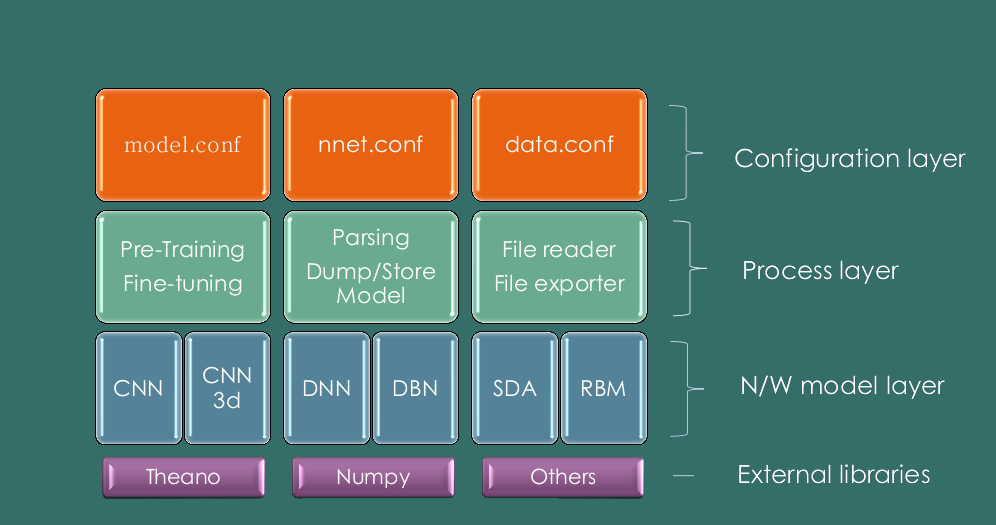
\includegraphics[width=1\textwidth]{./imgs/Python-DNNArch.png}
\end{figure}

\subsection{Salient Features}
\label{sec:python-dnnFeatures}
\begin{itemize}
\item Easy configuration of the models, configurations
are organised in JSON format and  hence make it legible to humans.
\item Run efficiently in CPU and GPU architectures.
\item Able to load the pre-trained model and dump the trained model.
\item Different types of Data Reader and Data Exporter.
\item Can be used as a standalone application as well as a standard  library.
\item Released in Apache Software License(version 2).\\
\end{itemize}

\section{Summary}
TODO............
%%%%%%%%%%%%%%%%%%%%%%%%%%%%%%%%%%%%%%%%%%%%%%%%%%%%%%%%%%%%%%%%%%%%%%%%%%%%%%%%%%%%%%%%%%%%%%%%%%%%%%%%%%%%%%%%%%%%%%%%
